\documentclass{article}
\usepackage{graphicx}
\usepackage[utf8]{inputenc}
\usepackage[T1]{fontenc}
\usepackage{hyperref} % Add this package
\usepackage{longtable} % For tables
\usepackage{booktabs}  % For tables
\usepackage{array}     % For tables
\usepackage{amsmath}

\title{Teoria Współbieżności \\ Zadanie Domowe - Sieci Petriego}
\author{Robert Mesek}
\date{}

\begin{document}

\maketitle

\section{Zadanie - Własna maszyna stanów}
\subsection{Reprezentacja sieci}
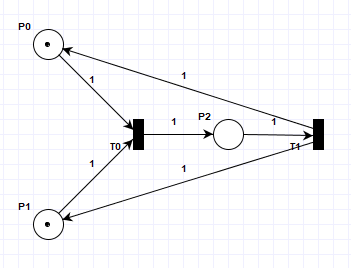
\includegraphics[width=\textwidth]{images/zadanie-1-1.png}
\subsection{Niezmienniki}
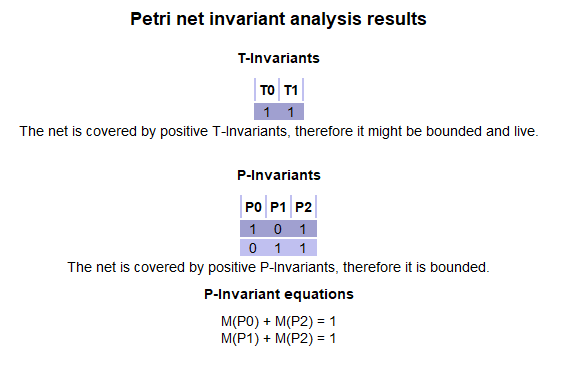
\includegraphics[width=\textwidth]{images/zadanie-1-3.png}
\subsection{Graf osiągalności}
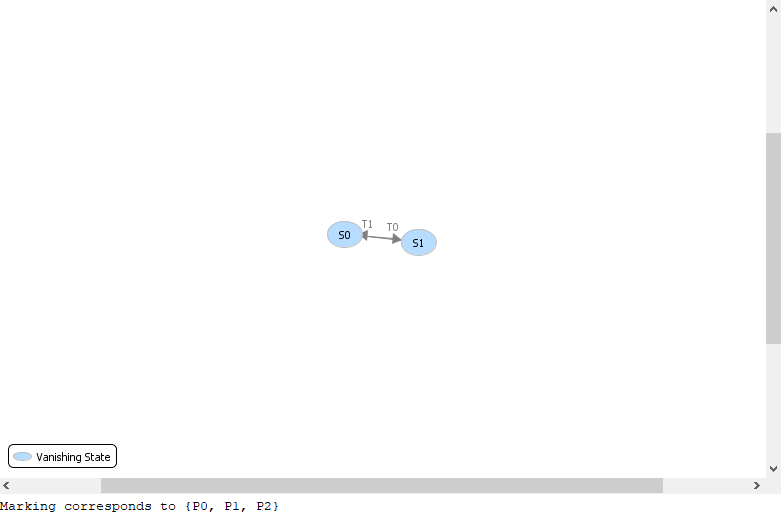
\includegraphics[width=\textwidth]{images/zadanie-1-2.png}

\section{Zadanie - Symulacja sieci}
\subsection{Reprezentacja sieci}
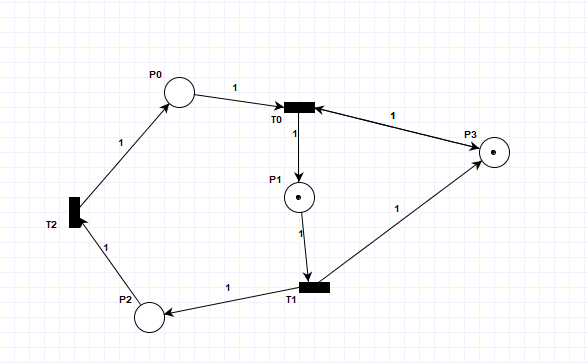
\includegraphics[width=\textwidth]{images/zadanie-2-1.png}
\subsection{Niezmienniki}
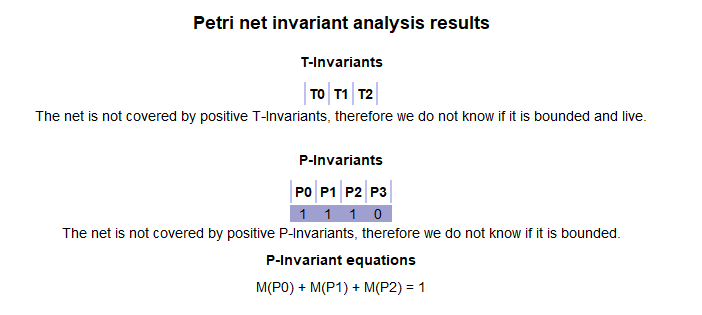
\includegraphics[width=\textwidth]{images/zadanie-2-2.png}
Na podstawie analizy tych niezmienników nie jesteśmy w stanie 
wyciągnąć żadnych wniosków.
\subsection{Graf osiągalności}
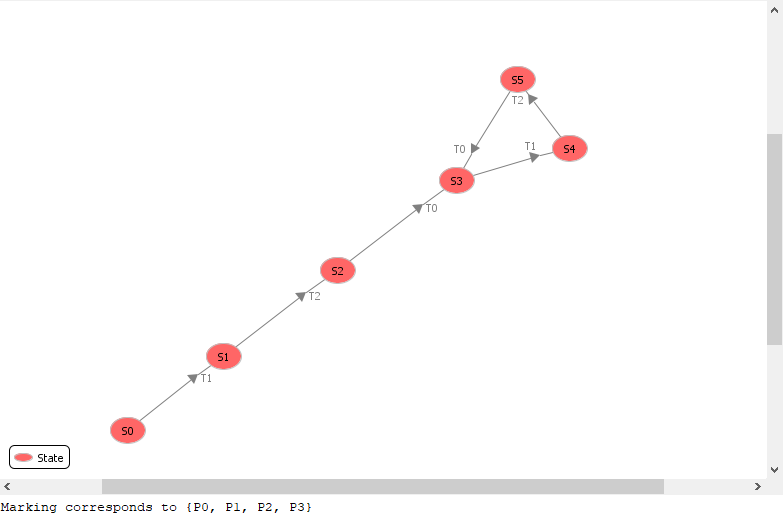
\includegraphics[width=\textwidth]{images/zadanie-2-3.png}
Możemy z tego grafu wywnioskować, że sieć jest żywa, ponieważ
z każdego stanu, możemy w pewnej liczbie kroków wykonać, 
każde z możliwych przejść ($T_0$, $T_1$, $T_2$).
\newline
Siec ta jest także ograniczona, ponieważ graf osiągalności
jest skończony.

\section{Zadanie - Dwa procesy}
\subsection{Reprezentacja sieci}
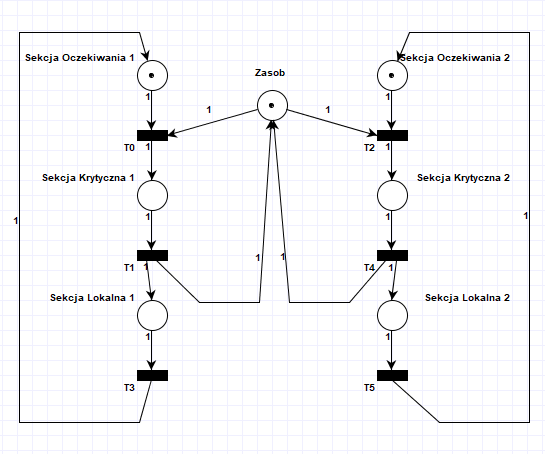
\includegraphics[width=\textwidth]{images/zadanie-3-1.png}
\subsection{Niezmienniki}
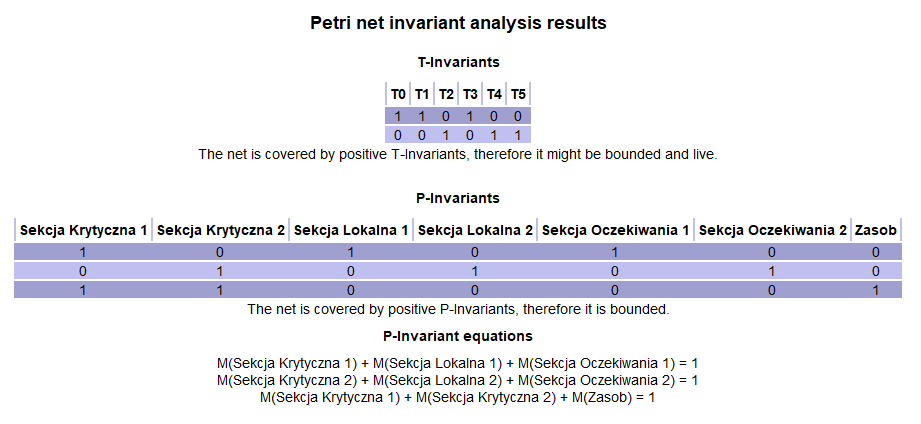
\includegraphics[width=\textwidth]{images/zadanie-3-2.png}
Ochronę sekcji krytycznej pokazuje ostatnie równanie:
\newline
$M(\text{Sekcja Krytyczna 1}) + M(\text{Sekcja Krytyczna 2}) 
+ M(\text{Zasób}) = 1$
\subsection{Graf osiągalności}
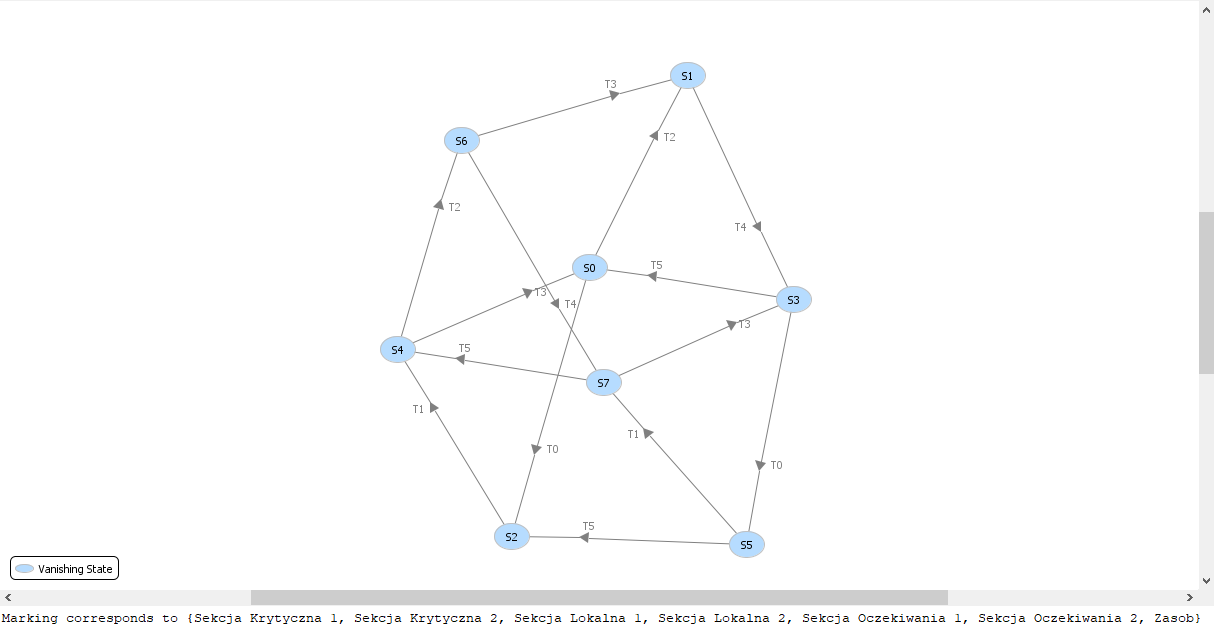
\includegraphics[width=\textwidth]{images/zadanie-3-3.png}
\subsection{Analiza stanów}
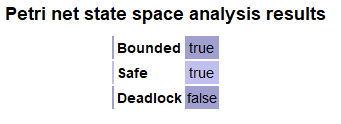
\includegraphics[width=0.75\textwidth]{images/zadanie-3-4.png}

\section{Zadanie - Producent i konsument z ograniczonym buforem}
\subsection{Reprezentacja sieci}
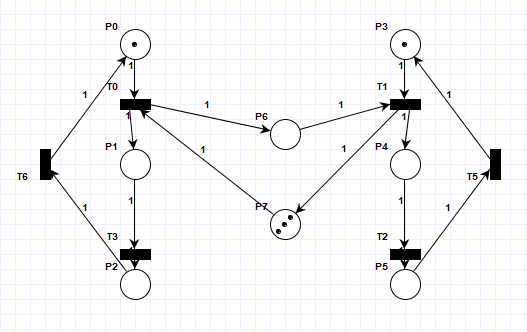
\includegraphics[width=\textwidth]{images/zadanie-4-1.png}
\subsection{Niezmienniki}
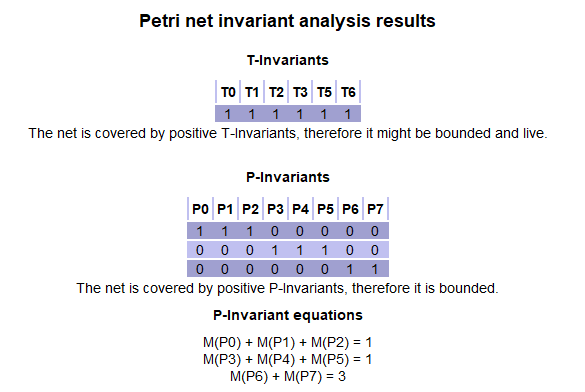
\includegraphics[width=\textwidth]{images/zadanie-4-2.png}
Sieć jest zachowawcza, ponieważ liczba tokenów w sieci pozostaje
stała.
\newline
O rozmiarze bufora mówi nam ostatnie równanie:
$M(\text{P6}) + M(\text{P7}) = 3$


\section{Zadanie - Producent i konsument z nieograniczonym buforem}
\subsection{Reprezentacja sieci}
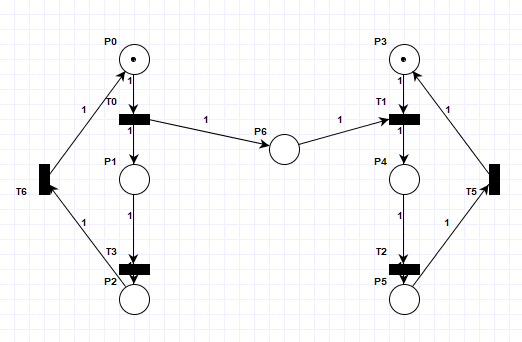
\includegraphics[width=\textwidth]{images/zadanie-5-1.png}
\subsection{Niezmienniki}
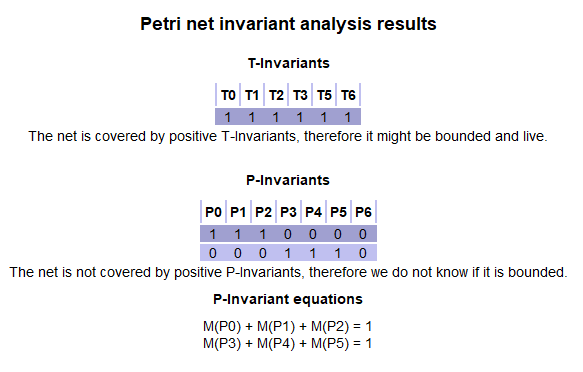
\includegraphics[width=\textwidth]{images/zadanie-5-2.png}

\section{Zadanie - Zakleszczenie}
\subsection{Reprezentacja sieci}
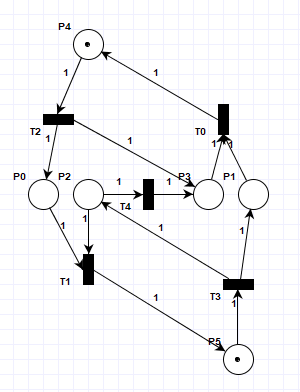
\includegraphics[width=\textwidth]{images/zadanie-6-1.png}
\subsection{Niezmienniki}
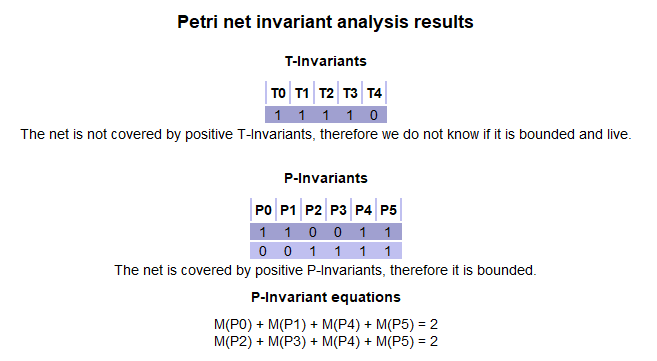
\includegraphics[width=\textwidth]{images/zadanie-6-2.png}
\subsection{Graf osiągalności}
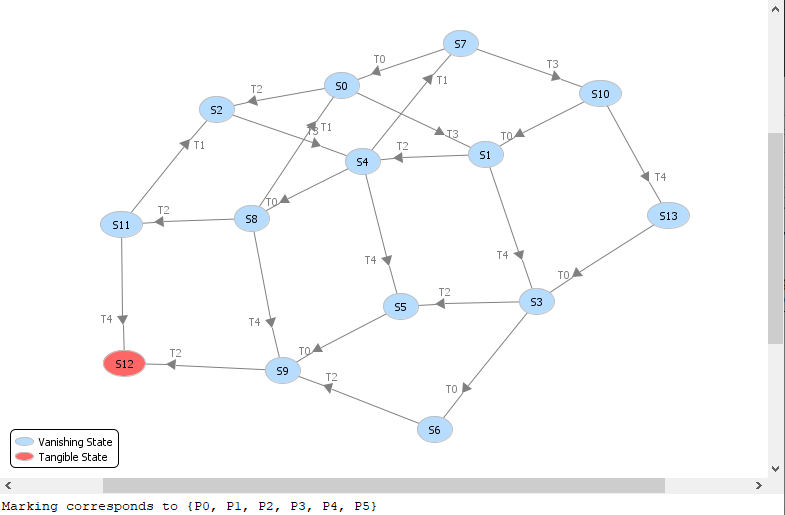
\includegraphics[width=\textwidth]{images/zadanie-6-3.png}
\subsection{Analiza stanów}
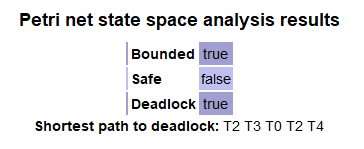
\includegraphics[width=0.75\textwidth]{images/zadanie-6-4.png}

\end{document}